\documentclass[12pt]{article}

\usepackage[margin=1in]{geometry}  % set the margins to 1in on all sides
\usepackage{graphicx}              % to include figures
\usepackage{amsmath}               % great math stuff
\usepackage{amsfonts}              % for blackboard bold, etc
\usepackage{amsthm}                % better theorem environments
\usepackage{url}

% various theorems, numbered by section

\newtheorem{thm}{Theorem}[section]
\newtheorem{lem}[thm]{Lemma}
\newtheorem{prop}[thm]{Proposition}
\newtheorem{cor}[thm]{Corollary}
\newtheorem{conj}[thm]{Conjecture}
\newtheorem{dfn}[thm]{Definition}

\DeclareMathOperator{\id}{id}

\newcommand{\bd}[1]{\mathbf{#1}}  % for bolding symbols
\newcommand{\RR}{\mathbb{R}}      % for Real numbers
\newcommand{\ZZ}{\mathbb{Z}}      % for Integers
\newcommand{\col}[1]{\left[\begin{matrix} #1 \end{matrix} \right]}
\newcommand{\comb}[2]{\binom{#1^2 + #2^2}{#1+#2}}
	

\begin{document}


\nocite{*}

\title{A Generalized Sphere Theorem for Positively Curved Combinatorial 3-Manifolds}

\author{Aaron Trout \\ Department of Mathematics \\
Chatham University \\ Woodland Rd, Pittsburgh PA 15232 USA \and
Vadas Gintautas\\ Department of Physics \\
Chatham University \\ Woodland Rd, Pittsburgh PA 15232 USA}


\maketitle

\begin{abstract}
The generalized sphere theorem of Grove and Shiohama is a central result in the differential geometry of positively curved manifolds. It shows that if $M$ is a Riemannian manifold whose sectional curvature is everywhere greater than a positive constant and $M$ has diameter greater than half the maximum allowed by the Bonnet-Myers theorem, then $M$ must be homeomorphic to a sphere. In this paper, we present a novel discrete version of this theorem which applies to positively curved {\em combinatorial} 3-manifolds. That is, those for which at most five tetrahedra are incident at each edge. In the standard piecewise-linear metric, this bound is equivalent to requiring an angle deficit along each edge. Such spaces have been studied previously and found to satisfy a beautiful discrete version of the Bonnet-Myers theorem. Here we prove a corresponding {\em discrete} generalized sphere theorem using a complete census of positively curved 3-manifolds completed by Lutz and Sullivan.
\end{abstract}


\section{Introduction}

Differential geometry is of central importance not only to geometers but also topologists, physicists and, increasingly, many of those interested in applied topics such as finite element analysis and computer graphics. One new offshoot in this area is {\em discrete differential geometry} (DDG) which seeks discrete analogues to the classical theorems and concepts from differential geometry. Since many computational treatments of differential geometry involve discretizing shapes, this subject has particular relevance for those with applied interests, see \cite{grinspun2006discrete} for examples. Other recent DDG work with a more pure-mathematics flavor can be found in \cite{BMM,Crowley,EMM,forman2,GGL1,GGL2,GGL3,stone}. 

A particularly important goal in classical differential geometry is to elucidate the relationship between the curvature of a Riemannian (or semi-Riemannian) space and its topology. The classical
results in this area are numerous, beautiful, and have inspired an
enormous amount of subsequent research. In this paper, we will present a discrete analogue of the ``generalized'' sphere theorem of Grove and Shiohama \cite{groveshiohama}.

\begin{thm}[Grove-Shiohama] Let $M$ be a complete, connected, $n$-dimensional Riemannian manifold with section curvature $K \geq \delta > 0$ and diameter greater than $\frac{\pi}{2\sqrt{\delta}}$. Then, $M$ is homeomorphic to a sphere.
\label{thm:grove_shiohama}
\end{thm}

\noindent Note that this bound is sharp, since the real projective space $\mathbb{RP}^n$ admits a metric with uniform sectional curvature $K=1$ and diameter $\pi/2$. We should also note also that the diameter bound in Theorem \ref{thm:grove_shiohama} is exactly half the maximum diameter allowed by the Bonnet-Myers theorem:

\begin{thm}[Bonnet-Myers] Let $M$ be a complete, connected, $n$-dimensional Riemannian manifold with sectional curvature $K \geq \delta > 0$. Then the diameter of $M$ is at most $\frac{\pi}{\sqrt{\delta}}$.
\label{thm:bonnet_myers}
\end{thm}

\noindent The main result of this paper is a discrete version of Theorem \ref{thm:grove_shiohama} which is proved by brute-force checking of a combinatorial 3-manifold census created by Lutz and Sullivan \cite{LS}. Before we can state precisely this result, we need a few preliminaries.

\section{Preliminaries}
\label{sect:basics}

The discrete version of Theorem \ref{thm:grove_shiohama} given in this paper will apply to positively curved combinatorial 3-manifolds. A \textbf{combinatorial 3-manifold} $M$ is an abstract simplicial complex in which the link of each vertex is a 2-sphere. We call such a space \textbf{positively curved} if at most five tetrahedra are incident along each edge. Why this terminology? If we endow $M$ with the standard piecewise-linear (PL) metric in which all edges have unit-length, this condition is equivalent to requiring an angle deficit along each edge. In classical differential geometry an angle deficit is intimately related to positive curvature.

A very natural discrete definition of distance in an abstract simplicial complex uses \textbf{edge-paths}. That is, paths entirely contained in the 1-skeleton of $M$. Let $\mathcal{P}_1$ denote the set of all edge-paths on $M$.

\begin{dfn}The \textbf{edge-distance} between two vertices $v$ and $w$ in an abstract simplicial complex $M$ is the minimum length (as a PL-path in the standard PL-metric) of an edge-path from $v$ to $w$. We denote this quantity $d_1(v,w)$. The \textbf{edge-diameter} of $M$, written as $diam_1(M)$, is the maximum of $d_1(v,w)$ over all pairs of vertices $v$ and $w$ in $M$. 
\end{dfn}

\noindent Note that the length of an edge-path is simply the number of edges it traverses.

A discrete version of the Bonnet-Myers theorem was previously proved in \cite{Trout10}. It applies to positively curved combinatorial 3-manifolds and gives a diameter bound in terms of the edge-diameter.

\begin{thm}[Trout] For any connected positively curved combinatorial 3-manifold $M$ we have $diam_1(M)\leq 5$. Moreover, this bound is sharp.
\label{thm:discrete_BM}
\end{thm}

\noindent Interestingly, while the statement of Theorem \ref{thm:discrete_BM} uses edge-diameter, its proof relies on expanding the set of paths under consideration to include those which contain not only edges, but also other types of PL-paths between vertices.

\subsection{Hops and Jumps}
The first new type of path is called a {\em hop}.

\begin{dfn}[Hops] Suppose $\tau$ is a 2-simplex in $M$ and $v_1$ and $v_2$ are vertices in $M$ such that $v_1*\tau$ and $v_2*\tau$ are 3-simplices in $M$. The PL-path from $v_1$ through the barycenter of $\tau$ and ending on $v_2$ will be called a \textbf{hop} from $v_1$ to $v_2$. See Figure \ref{fig:hop} for an illustration.
\end{dfn}

\begin{figure}
	\centering
		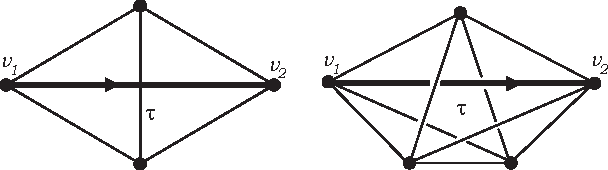
\includegraphics[width=0.23\linewidth]{figures/hops.pdf}
    \caption{A {\em hop} from vertex $v_1$ to vertex $v_2$.}
    	\label{fig:hop}
\end{figure}

\noindent The other new type of path we call a {\em jump.}

\begin{dfn}[Jumps] Suppose there are edges $e_1$ and $e_2$ and vertices $v_1$ and $v_2$ in $M$ so that $e_1*e_2$ is a 3-simplex in $M$ and $v_1*e_1$ and $v_2*e_2$ are 2-simplices in $M$. We call the PL-path from $v_1$ through the barycenters of $e_1$ and $e_2$ and ending on $v_2$ a \textbf{jump} from $v_1$ to $v_2$. For an illustration, see Figure \ref{fig:jump}.
\end{dfn}

\begin{figure}
	\centering
		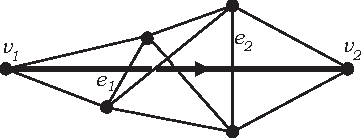
\includegraphics[width=0.30\linewidth]{figures/jump.pdf}
    \caption{A {\em jump} from vertex $v_1$ to vertex $v_2$}
    \label{fig:jump}
\end{figure}

Just as for edges in an edge-path, the length of each hop and jump will be its length as a PL-path in the standard PL metric. Some Euclidean geometry tells us these lengths are \begin{equation} \label{eqn:jump_length} H = \frac{2}{3}\sqrt{2} \end{equation} and \begin{equation} \label{eqn:jump_length} J = \frac{1}{2}\sqrt{2} + \sqrt{3} \end{equation} respectively. We let $d(v,w)$ denote the \textbf{distance between vertices $v$ and $w$} obtained by minimizing over all paths containing edges as well as hops and jumps. Similarly, we let $diam(M)$ denote the \textbf{diameter of $M$} defined in terms of the distance function $d$. Let $\mathcal{P}$ denote the set of all the paths containing edges, hops or jumps.

Why are these paths relevant to this paper? In the classical setting, the generalized sphere theorem requires a manifold to have diameter more than half the maximum allowed by the Bonnet-Myers theorem, and this diameter bound cannot be improved. If we naively imitate the classical results in the discrete setting, from Theorem \ref{thm:discrete_BM} we would want to assume the bound $diam_1(M)>\frac{5}{2}$. Unfortunately, there are positively curved combinatorial 3-manifolds with edge-diameter three that are not homeomorphic to the 3-sphere. In particular, as we will see, $\mathbb{RP}^3$ has positively curved triangulations with edge-diameter three. However, if we instead use the finer-grained measure of diameter, $diam(M)$, the problem disappears and the discrete results mirror the classical ones exactly. That is, we can prove a discrete version of the generalized sphere theorem with a diameter bound exactly half the maximum allowed by the corresponding discrete Bonnet-Myers theorem.

What is the discrete Bonnet-Myers theorem corresponding to Theorem \ref{thm:discrete_BM} but which uses $diam(M)$? From the proof of Theorem \ref{thm:discrete_BM} in \cite{Trout10}, we have the following bound on the possible distances which occur in a positively curved 3-manifold.

\begin{lem}[Trout] If $v$ and $w$ are vertices in a connected positively curved combinatorial 3-manifold $M$ then $d(v,w) \in \{0, 1, H, 2, J, 3, 2H, 4, 2J \}$.
\end{lem}

\noindent Note that we have listed the possible distances in increasing numerical order. This result implies the desired discrete Bonnet-Myers type theorem.

\begin{thm}[Trout] For any connected positively curved combinatorial 3-manifold $M$ we have $diam(M) \leq 2J$.
\label{thm:discrete_BM_expanded_paths}
\end{thm}

\noindent Note, it is shown in \cite{Trout10} that this diameter bound is sharp.

\section{Main Results}

We are now able to state our main result.

\begin{thm} Any connected positively curved combinatorial 3-manifold $M$ with $diam(M)>J$ is homeomorphic to the 3-sphere. This bound is sharp, and equal to half the maximum diameter which occurs for any such $M$.
\label{thm:discrete_GS}
\end{thm}

\noindent The proof of this theorem relies on the remarkable work of Lutz, Sullivan and Sulanke in \cite{Lutz07, LutzSul_unpub, sulanke2009isomorphism} who created a complete census of positively curved combinatorial 3-manifolds along with a list of their topological types, see \cite{Lutz_online_manifolds} and \cite{Lutz_online_topological_types}. This census contains 4787 manifolds, with the following topologies represented: the 3-sphere $S^3$, the real projective space $\mathbb{RP}^3$, the lens spaces $L(3,1)$ and $L(4,1)$, and the cube space $S^3/Q$. Note that all of these manifolds are homeomorphic to either a 3-sphere or to the quotient space of a 3-sphere under the action of a finite group. 

A small Python program was created to examine each manifold in the census and compute its diameter. See Figure \ref{fig:global_statistics} for a plot of the number of manifolds by topological type and diameter. As claimed, every manifold with diameter greater than $J$ is a 3-sphere. The corresponding data using the coarser-grained edge-diameter can be found in Figure \ref{fig:global_statistics_edges}. Note that there are $3$-manifolds homeomor

\begin{figure}
    \begin{center}
    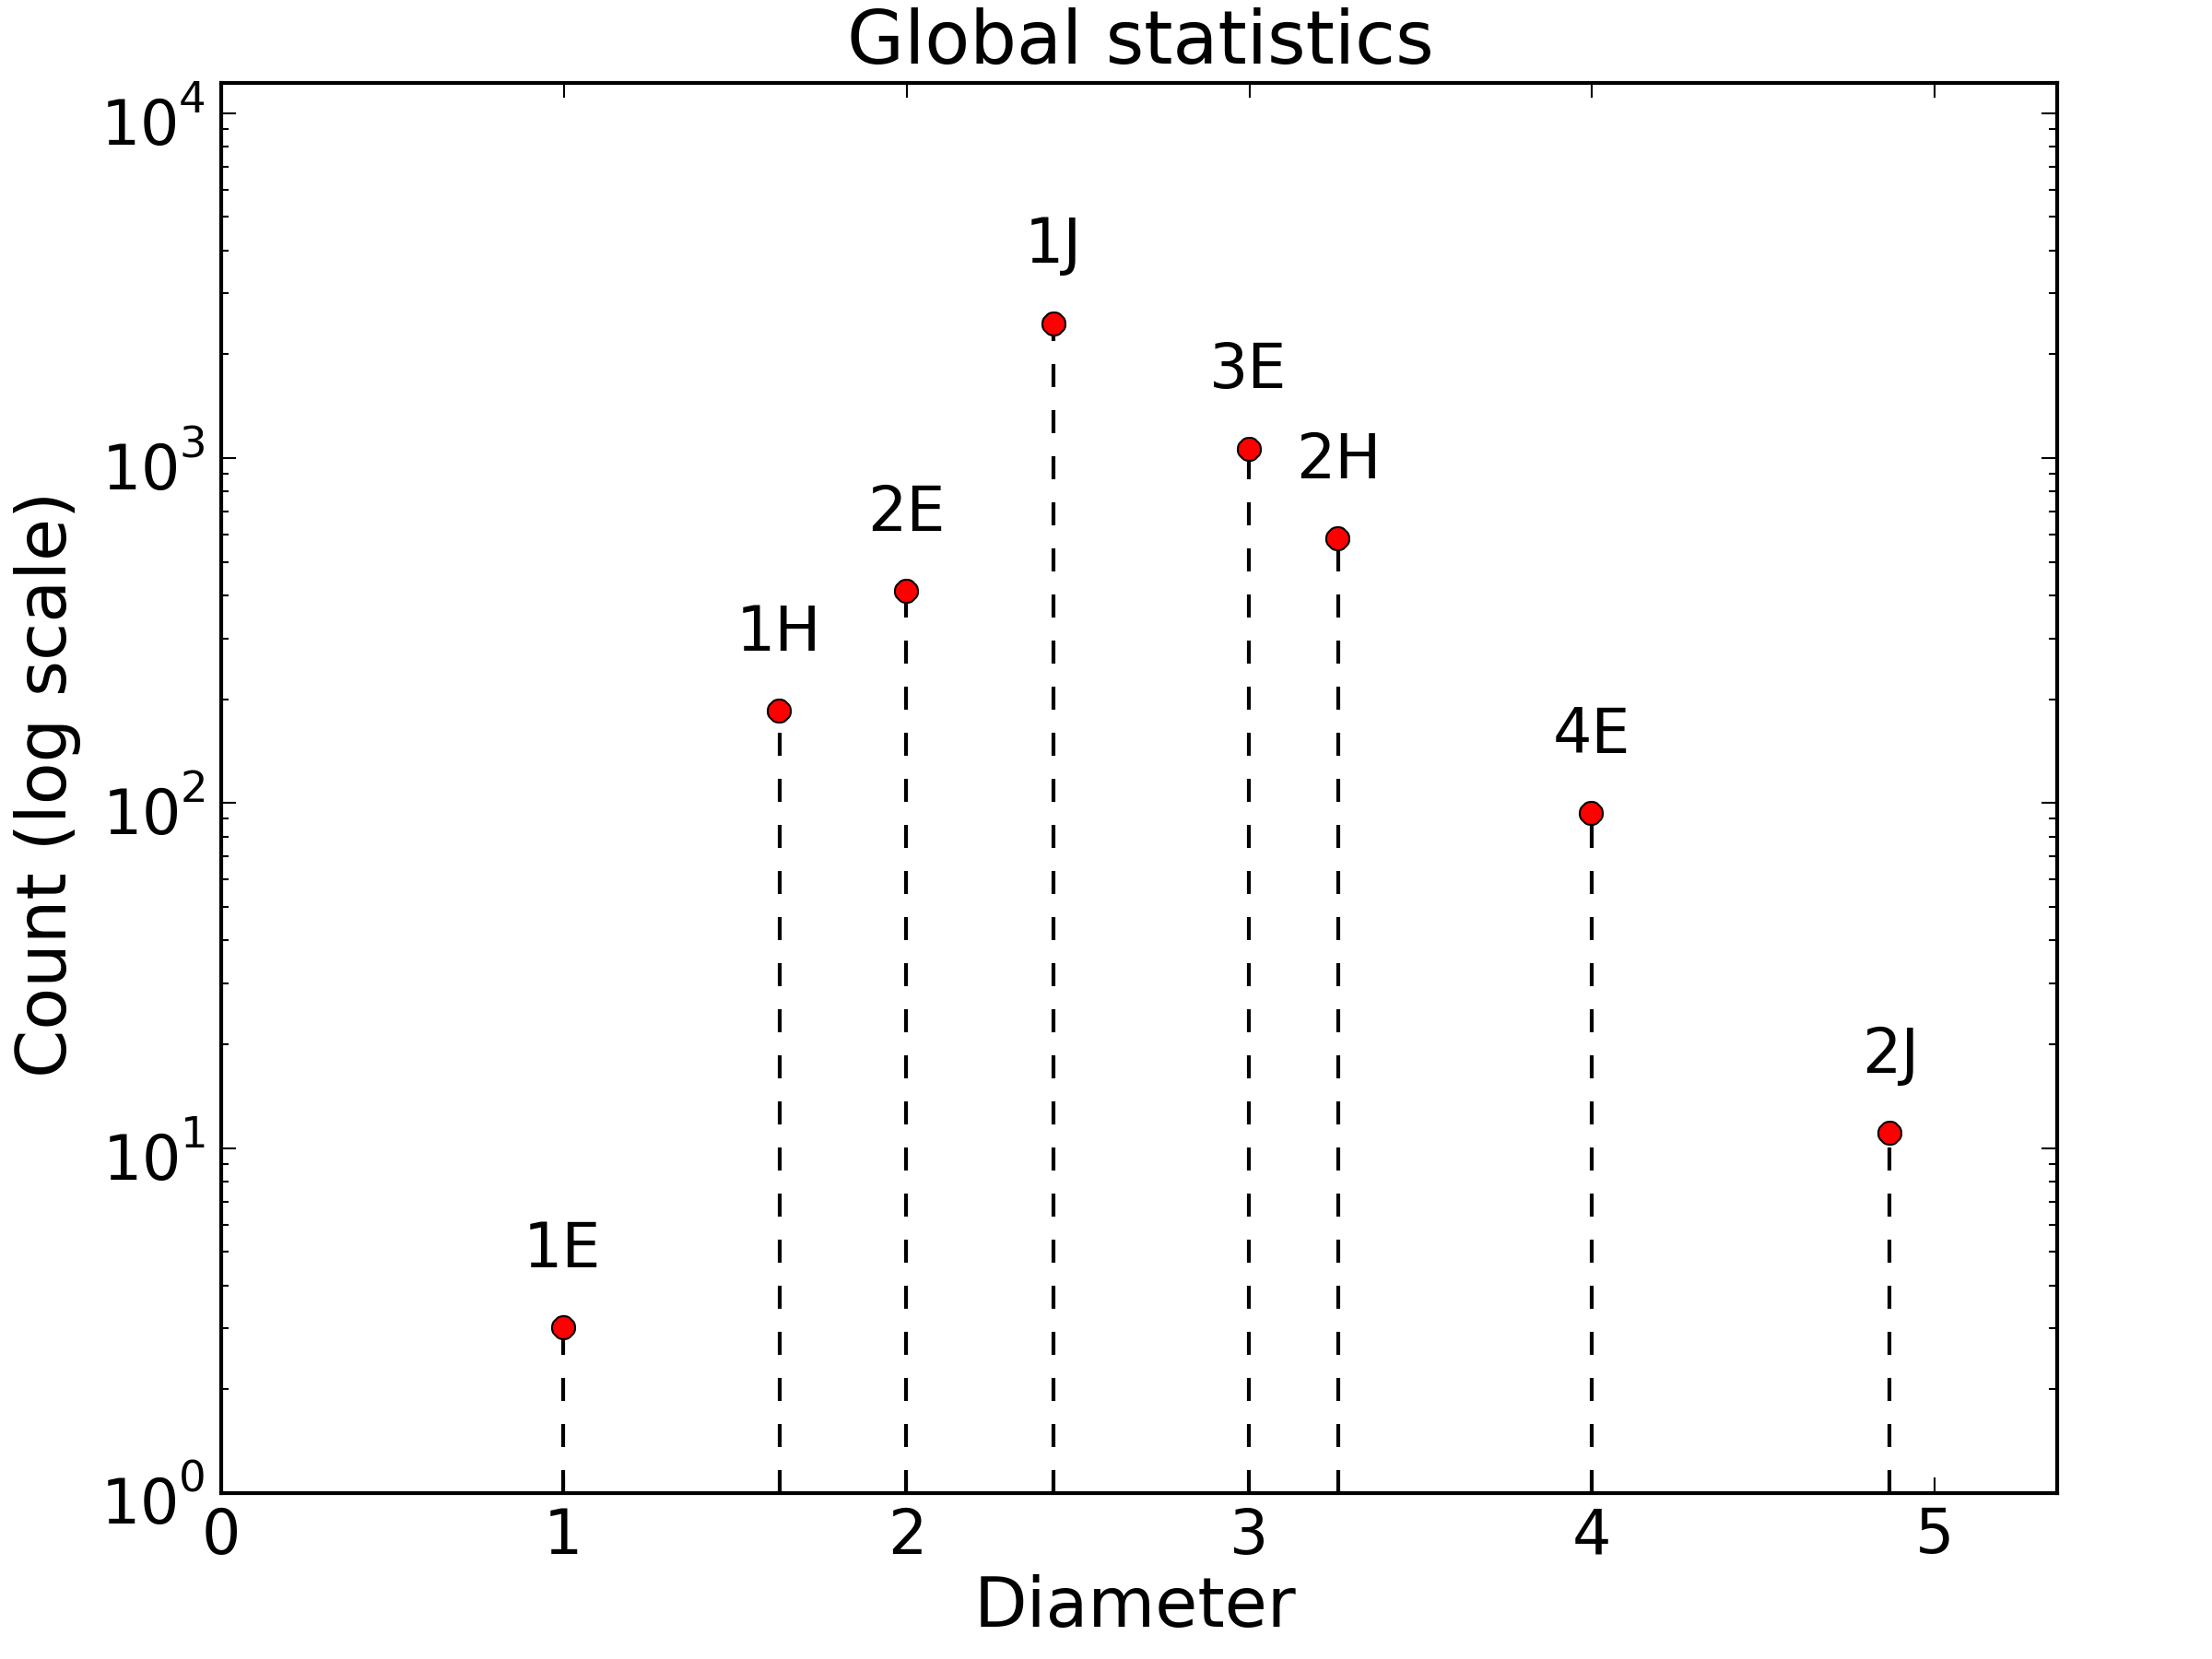
\includegraphics[width=0.6\linewidth]{figures/global_statistics.png}
    \caption{Global statistics. TO DO: CHANGE DIAMETER LABELS TO $1, H, 2, J, 3, 2H, 4, 2J$ AND PUT THESE ON HORIZONTAL AXIS. TO DO: CHANGE GRAPH TO SHOW SEPARATE DATA POINTS FOR EACH TOPOLOGICAL TYPE. TO DO: CREATE ANOTHER GRAPH WITH JUST EDGE DIAMETER COUNTS}
    \end{center}
    \caption{TO DO: ADD CAPTION}
    \label{fig:global_statistics}
\end{figure}

\begin{figure}
    \begin{center}
    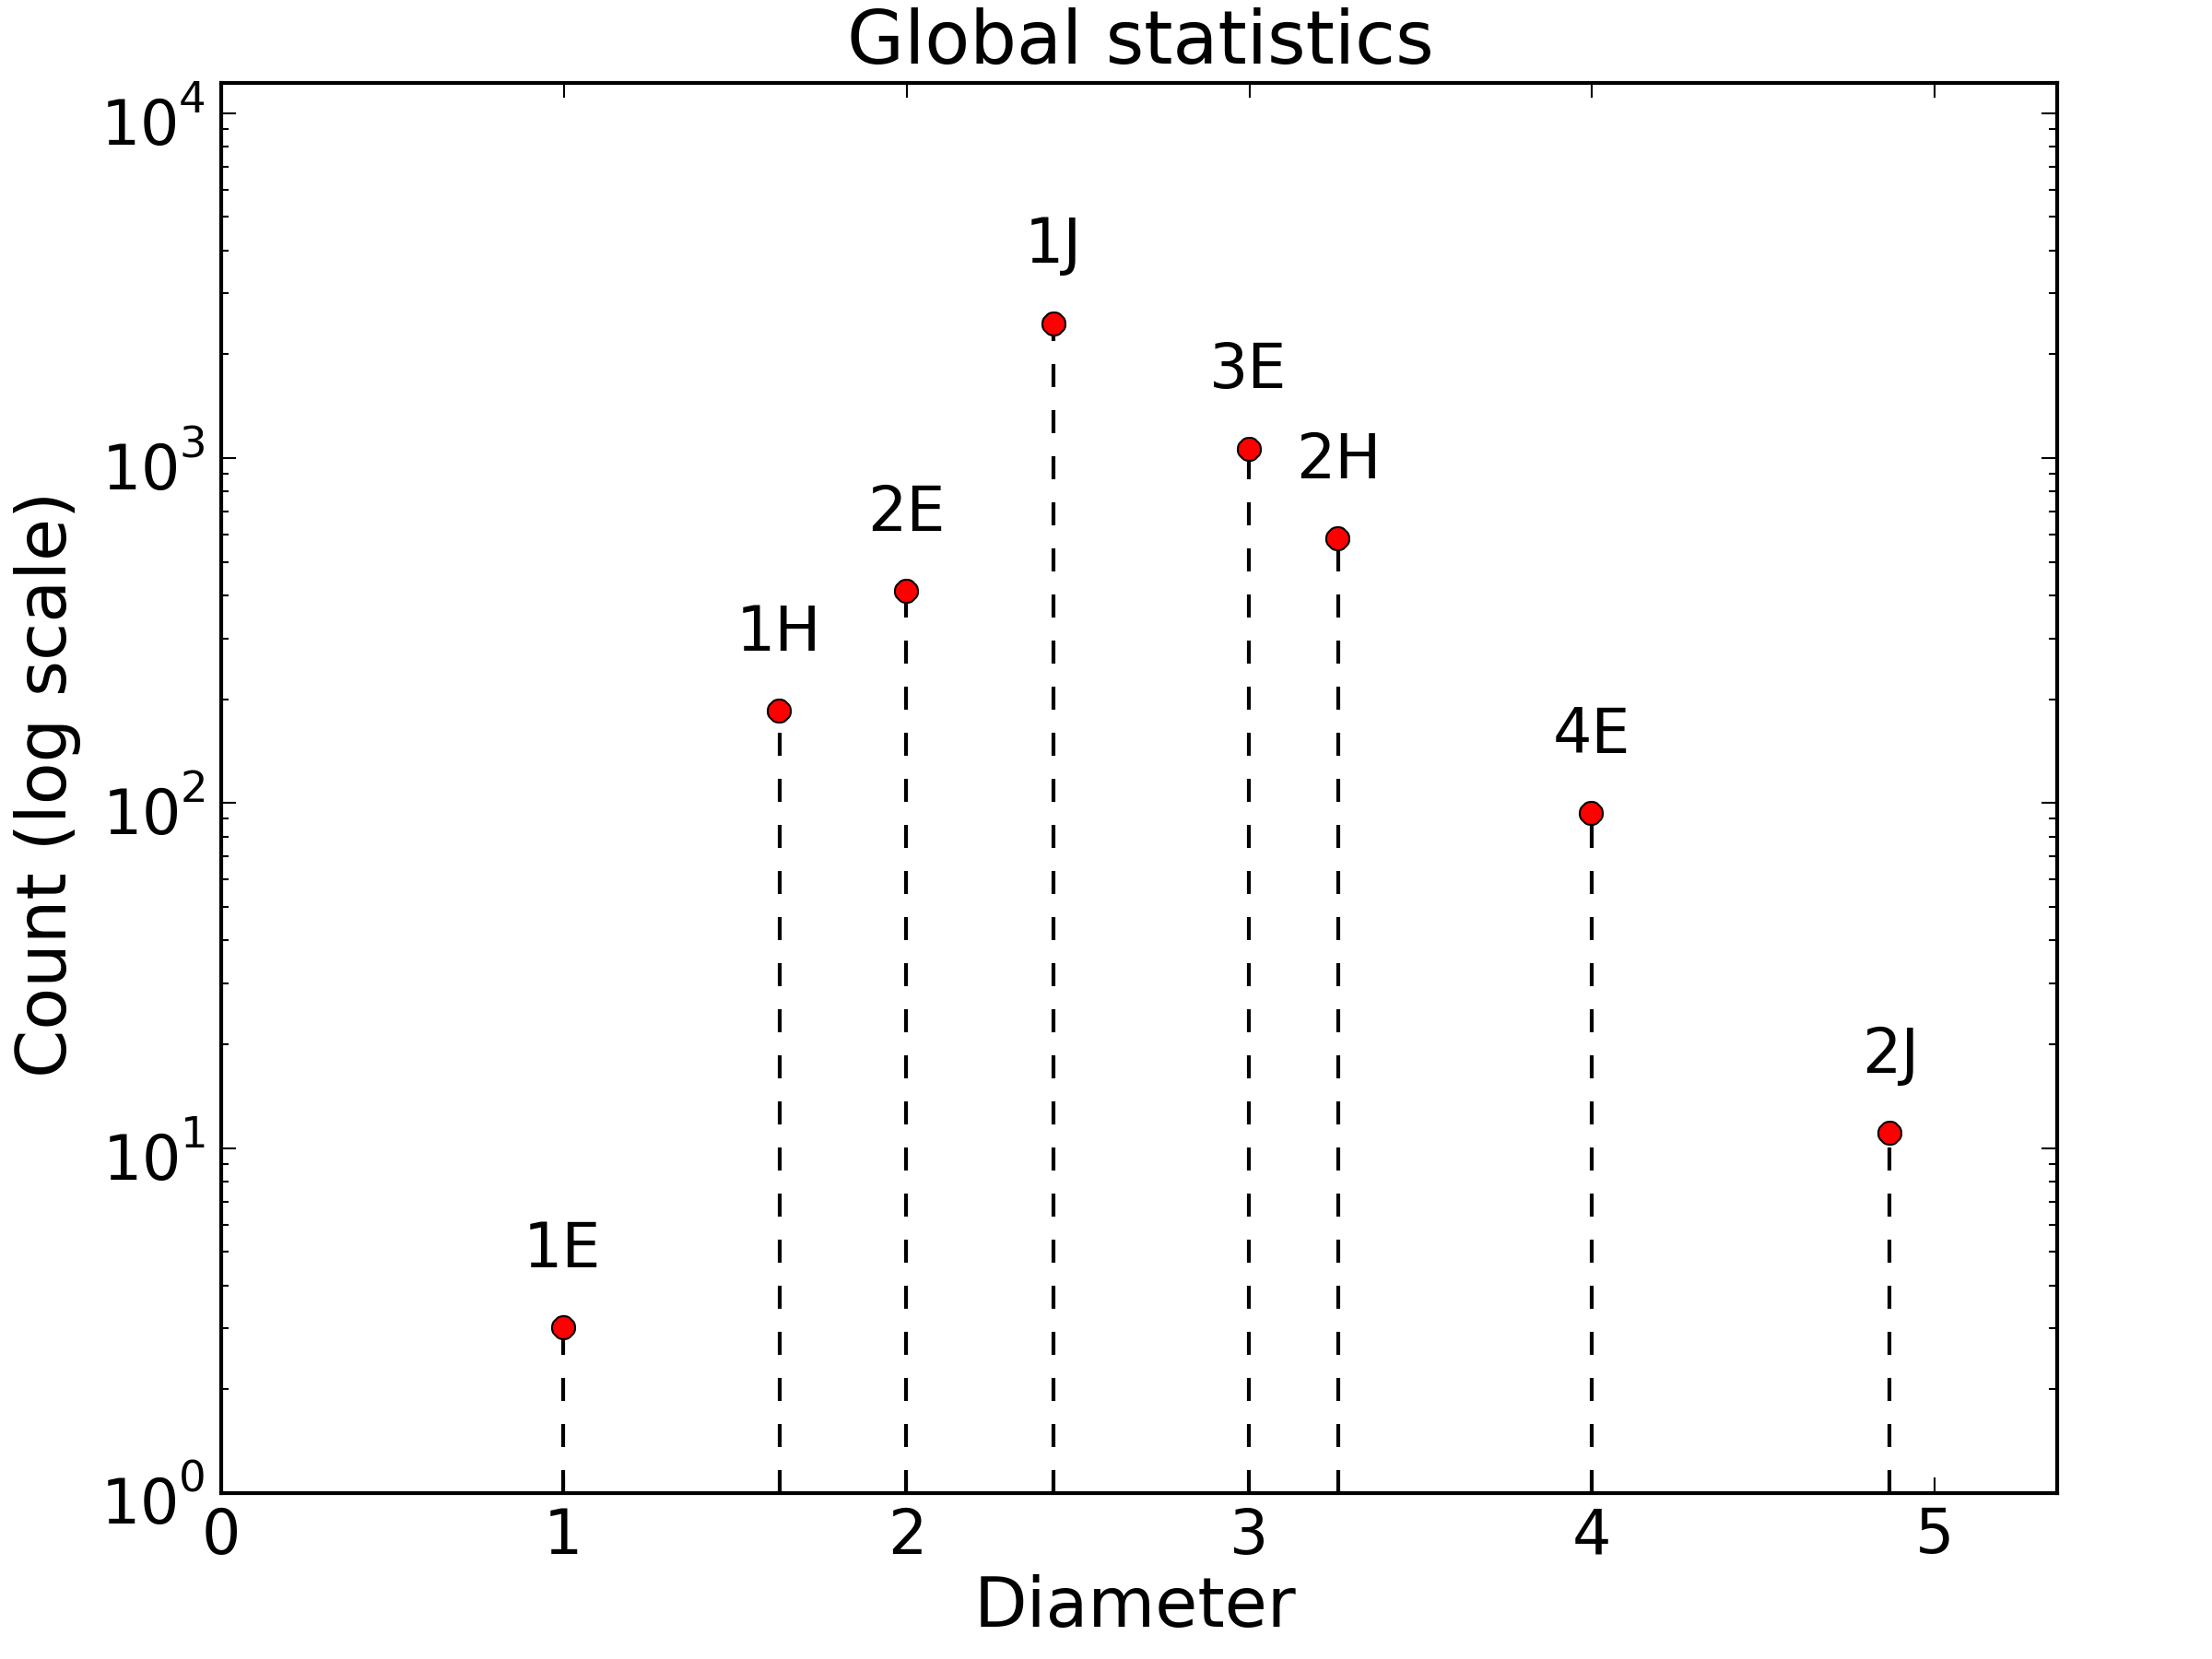
\includegraphics[width=0.6\linewidth]{figures/global_statistics.png}
    \end{center}
    \caption{TO DO: ADD CAPTION}
    \label{fig:global_statistics_edges}
\end{figure}

\begin{figure}
\centering
\begin{tabular} {| r | r | r | r | r | r | r |}
\hline
Diameter & $S^{3}/Q$ & $L(4,1)$ & $L(3,1)$ & $RP^{3}$ & $S^{3}$ & Total \\
\hline
\hline
$1$&  &  &  &   &3    & 3    \\
$H$&1 &  &  &10 &173  & 184  \\
$2$&  &  &1 &7  &401  & 409  \\
$J$&  &1 &1 &5  &2438 & 2445 \\
$3$&  &  &  &   &1060 & 1060 \\
$2H$&  &  &  &   &582  & 582  \\
$4$&  &  &  &   &93   & 93   \\
$2J$&  &  &  &   &11   & 11   \\
\hline
Total&1 &1 &2 &22   &4761   &4787  \\
\hline
\end{tabular}
\caption{The positively curved combinatorial 3-manifolds by diameter and topological type}
\label{fig:manifold_counts}
\end{figure}

\begin{figure}
\centering
\begin{tabular} {| r | r | r | r | r | r | r |}	
\hline
Diameter & $S^{3}/Q$ & $L(4,1)$ & $L(3,1)$ & $RP^{3}$ & $S^{3}$ & Total \\
\hline
\hline
$1$ &  &  &  &   &3    & 3    \\
$2$ & 1&  &1 &17 &574  & 593  \\
$3$ &  &1 &1 &5  &3498 & 3505 \\
$4$ &  &  &  &   &675  & 675   \\
$5$ &  &  &  &   &11   & 11   \\
\hline
Total&1 &1 &2 &22   &4761   &4787  \\
\hline
\end{tabular}
\caption{The positively curved combinatorial 3-manifolds by edge-diameter and topological type}
\label{fig:manifold_counts_edges}
\end{figure}

\section{Algorithm Used}

TO DO: BRIEF DISCUSSION OF ALGORITHM USED

\section{Discussion}
Why does adding additional paths above and beyond edge-paths restore the classical structure to our proof?


We should mention another notable advantage of expanding the space of paths to include hops and edges. In classical differential geometry, the starting point, the initial direction, and length completely determine a geodesic. There is no branching of geodesics. This property of fundamental importance to many proofs in Riemannian geometry. If we use only edge-paths, then in a positi`vely curved combinatorial 3-manifold it is possible to have two minimal paths with the same length and which begin by traversing the same edge, yet reach distinct destination vertices. That is, using only edge paths, minimal geodesics can ``branch''.

This important property is restored, at least for positively curved manifolds, if we include hops and jumps. In \cite{Trout10} the following is shown.

\begin{thm}(Unique Extension) If two minimal paths $P_1$ and $P_2$ in $\mathcal{P}$ pass through the same first two simplices of a positively curved 3-manifold $M$ and $P_1$ and $P_2$ have the same length, then $P_1 = P_2$. This result is false if $\mathcal{P}$ is replaced by $\mathcal{P}_1$.
\end{thm}

\bibliographystyle{plain}
\bibliography{manifolds}
\end{document}
